\section{Visualisierungen}
In diesem Kapitel werden die Anwendungsaufgaben die zu lösen sind analysiert und deren Lösung erklärt. Dabei werden zuerst die Anforderungen festgestellt und diese dann in Bezug auf die Präsentation und Interaktion der Visualisierungen angewandt.  

\subsection{Analyse}

Das Ziel der Visualisierungen ist es die \textit{World Happiness Report} Daten intuitiv und einfach zugänglich zu machen und es der Zielgruppe zu ermöglichen Länder und deren Ranking zu identifizieren. Auch einzelne Länder und deren Variablen sollen schnell zugänglich sein. Zudem sollen sie in der Lage sein Zusammenhänge in den Daten identifizieren zu können und die zeitliche Entwicklung der Daten zu verfolgen. \\

Hierfür ist es entscheidend, die einzelnen Anwendungsaufgaben durch verschiedene Visualisierungen abzudecken und möglichst klar die benötigten Informationen zu vermitteln. 
Am sinnvollsten ist es vermutlich mit einem Überblick in die Daten also einer allgemeineren Visualisierung zu beginnen um einen Eindruck für die Daten und deren Zusammenhänge zu vermitteln. \\

\subsection{Anforderungen}
Die Anforderungen an die Visualisierungen sind vielfältig. Sie werden fallen für jede der Zielprobleme leicht unterschiedlich aus. Allgemein ist die Anforderung einfach verständliche Visualierungen zu verwenden, welche wenig bis gar kein Hintergrundwissen über Datenvisualisierungsmethoden erfordern. Damit fallen bereits einige Methoden weg. Die Anforderungen werden nach Visualisierungszielen auf die drei Vorgegebenen Visualisierungen verteilt.\\

1st vis: größen vergleichen, lesbarkeit, Ländergruppen und Länder identifizieren, Muster sichtbar machen

2nd vis: Alle Variablen für ein Land auf einem Blick, Suche eines Landes, Einordnung im Vergleich zum Datenraum. 

3rd: historische daten imKontext anzeigen, entwicklungen sichtbar machen, vergleich ermöglichen. 

Um die Länder und deren erfasste Variablen miteinander Vergleichen zu können muss ein Auswahl von Variablen und Identifizierung der Länder möglich sein. Dies liegt daran das sich 6 Variablen kaum visuell deutlich gleichzeitig für alle Länder darstellen lassen. Daher ist es sinnvoller jeweils nur ein oder zwei Attribute darzustellen. Dies soll durch Nutzerinteraktion geschehen. \\

Um auch einen direkten Vergleich aller Attribute zu ermöglichen ist es sinnvoll die Möglichkeit zu bieten jeweils nur ein Land zu betrachten, für dieses jedoch alle Attribute zu zeigen. Hier muss auf einen Blick erkennbar sein wie die Attribute zueinander aufgestellt sind. Auch hier muss Nutzerinteraktion ermöglicht werden um alle Länder in dieser Weise einzeln zu betrachten. \\

\subsubsection{Visualisierung 1: Scatterplot}

Der Scatterplot soll möglich Muster in den Daten aufzeigen können und die Verteilung der Länder sichtbar machen. Um dies für alle Dimensionen zu ermöglichen lassen sich die X und Y - Achse durch die Dropdown Menüs anpassen. so lassen sich zwei Größen direkt miteinander Vergleichen. Zusätzlich sind die Punkt nach Länderregionen, welche im Datensatz gegeben waren, eingefärbt. Die Legende über dem Plot beschreibt welche Farbe welche Region darstellt. So lassen sich auch Muster in Bezug auf die Ländergruppen identifizieren. \\

\begin{figure}[h]
 \centering
 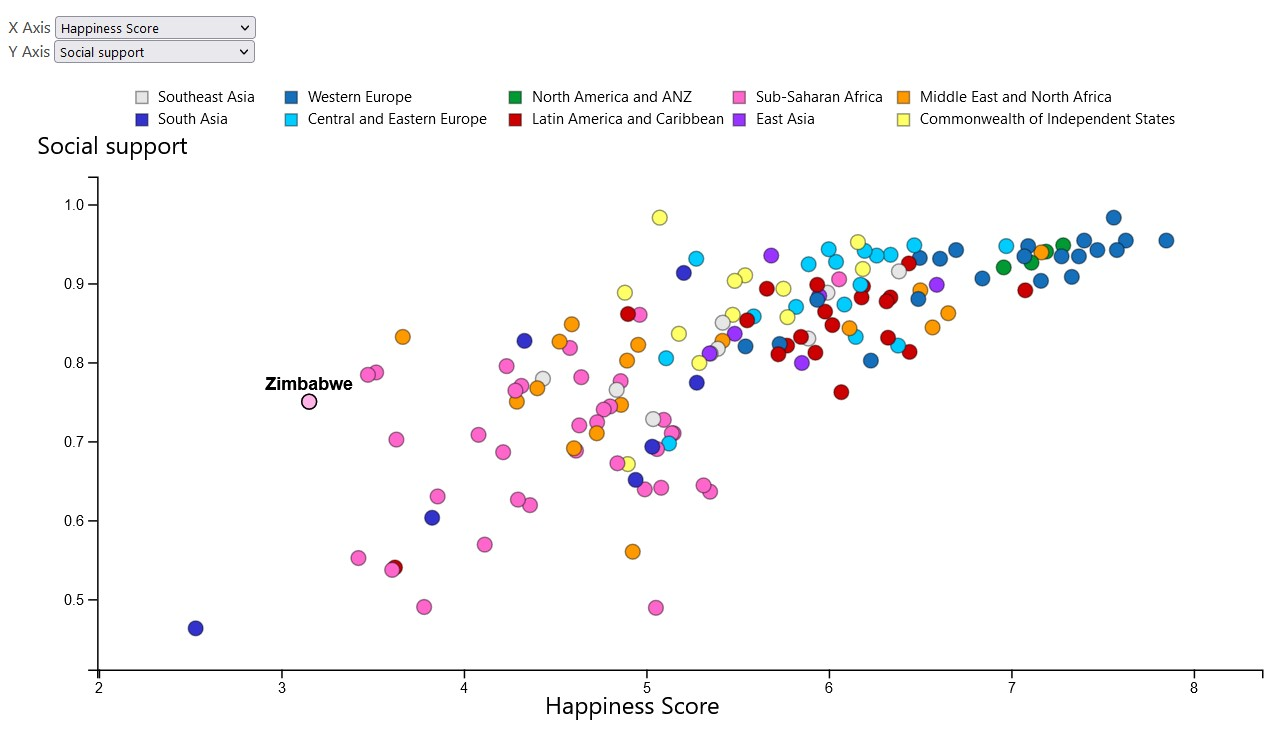
\includegraphics[width = \textwidth]{img/scatterplot.jpg}
 \caption{Scatterplot mit Bedienelementen}
 \label{fig:scatterplot}
\end{figure}

Möchte man einen Punkt identifizieren kann man mit dem Mauszeiger über diesem schweben, dann erscheint wie in Abbildung \ref{fig:scatterplot} der Landesname über dem Punkt. In diesem Beispiel ist es Zimbabwe. 


\subsubsection{Visualisierung 2: Polarplot}

Der Polarplot soll es ermöglichen alle Details über ein Land auf einen Blick sichtbar zu machen. Alle Dimensionen befinden sich auf im Kreis angeordneten Achsen. Diese sind dabei jeweils auf die verschieden Größen skaliert und mit Beschriftungen versehen. Das Maximum der jeweiligen Gruppe liegt dabei jeweils am Kreisrand. So lässt sich jedes Land schnell einordnen. \\

Der Happiness Score wird hier nicht innerhalb des Plots abgebildet. Er wird in Textform unter dem augewählten Land angezeigt, wie in Abbildung \ref{fig:polarplot} zu sehen. Der Polarplot ist vermutlich eine Darstellung die nicht jeder schoneinmal gesehen hat, allerdings ist die Strukur sehr simpel gehalten worden. Die visuelle Klarheit sollte es den Nutzer leicht machen die Daten schnell erfassen zu können. \\

\begin{figure}[h]
 \centering
 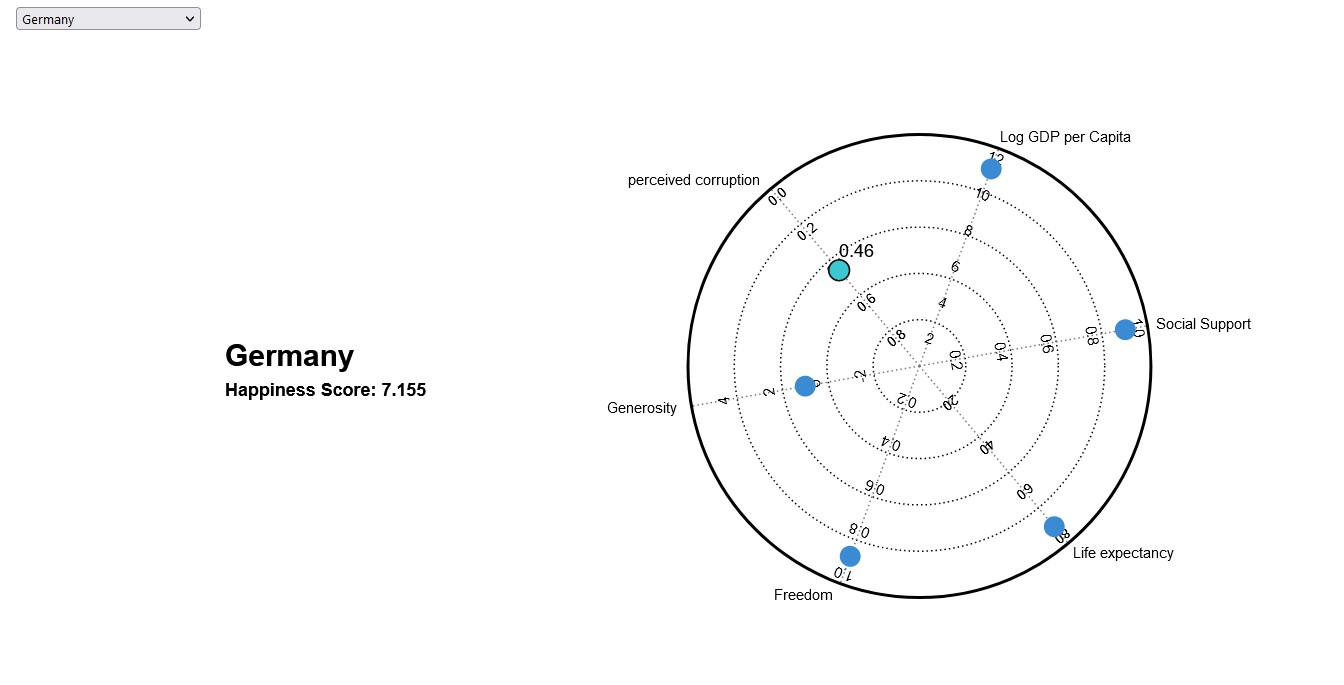
\includegraphics[width = \textwidth]{img/polarplot.jpg}
 \caption{Polarplot mit Bedienelementen}
 \label{fig:polarplot}
\end{figure}


Eine Alternative Visualisierung währen hier Parallel Koordinaten gewesen. Diese sind auch in der Lage mehrere Dimensionen gleichzeitig darzustellen. Allerdings sind sie visuell möglicherweise etwas unklarer, die verbundenen Punkte auf den verschiedenen Achsen suggerieren eine Abfolge oder einen festen Zusammenhang dieser. Das ist für diesen Polarplot nicht der Fall. Ein möglicher Vorteil des Parallelplots ist Möglichkeit viele Instanzen, in diesem Fall Länder, gleichzeitig darzustellen. Je nach Einstellung der Verbindungslinien lässt sich dann auch eine Verteilung ausmachen. 

\subsubsection{Visualisierung 3: Zeitreihe}

Die letzte Darstellung verwendet den zweiten Datensatz aus dem World Happiness Report auf Kaggle. Hier werden die historischen Daten dargestellt. Der Nutzer hat die Möglichkeit hier eine Größe zweier Länder zeitlich zu betrachten. Dies ermöglicht den Vergleich der Länder über einen Zeitraum von ca. 15 Jahren. Es lässt sich hier ein Eindruck darüber zu gewinnen wie statisch die verschiedenen Größen in verschiedenen Ländern verhalten. \\

Hier gibt es kaum andere Möglichkeiten diese Zeitliche Entwicklung darzustellen. Möglicherweise hätte man die Jahreswerte auch mittels eines Balkendiagrammes für die jeweils ausgewählten Länder darstellen können. Allerdings wird hier der Zusammenhang, beziehungsweise die zeitliche Entwicklung nicht klar dargestellt. 

\begin{figure}[h]
 \centering
 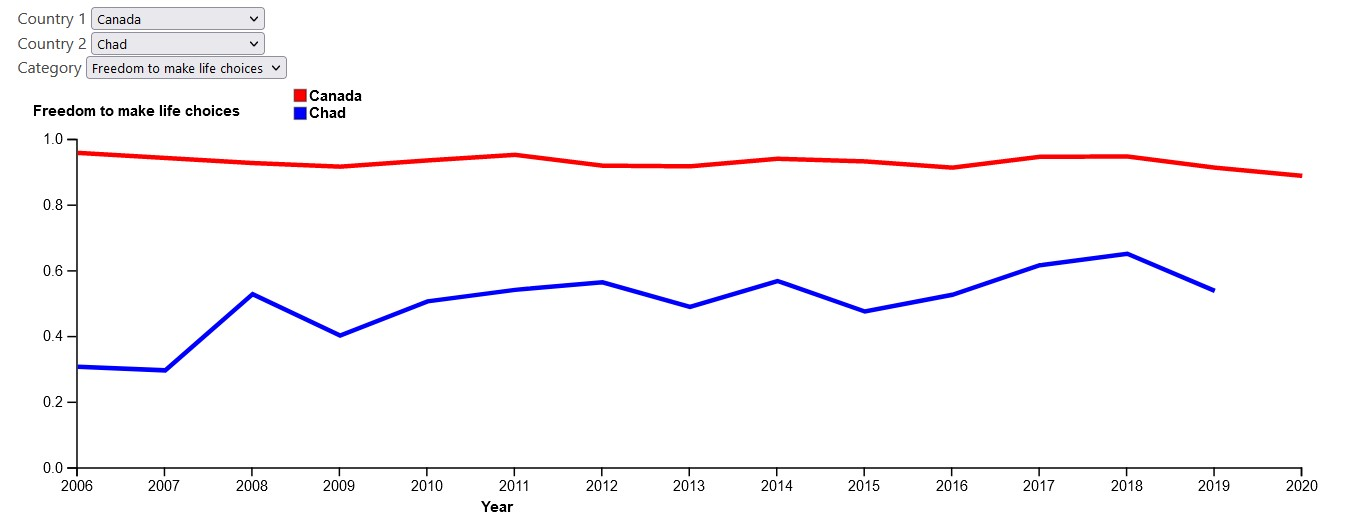
\includegraphics[width = \textwidth]{img/timeseries.jpg}
 \caption{Zeitreihe mit Bedienelementen}
 \label{fig:timeseries}
\end{figure}

Zu beachten ist bei dieser Darstellung, dass sie mit etwas unvollständigen Daten arbeitet. Die beiden vorherigen Darstellungen haben für jedes Land und jede Größe einen Wert. Hier fehlen bei einigen Länder Werte in einigen Jahren. Die fehlenden Jahre wurden hier durch das Zeichnen der Linien interpoliert. Dadurch haben alle Länder ununterbrochene Linien, sie starten und Enden aber in unterschiedlichen Jahren. Es wurde keine Extrapolation durchgeführt um Jahre zu ergänzen. Jedoch sind hier auch zwei weitere Größen verfügbar welche im ersteen Datensatz nicht enthalten sind. \textit{Positive Affect} und \textit{Negative Affect}. Sozusagen die Stimmung des jeweiligen Landes. Leider waren diese für die Durchschnitte nicht gegeben. Von einer nachträglichen ergänzung wurde abgesehen. 

\subsection{Interaktion}

Der Scatterplot weist die meisten Interaktionsmöglichkeiten auf. Es lassen sich beide Achsen vom Nutzer anpassen um die dort angezeigten Größen zu verändern, dies passiert über die Dropdown Menüs über dem Plot. Bewegt ein Nutzer seinen Mauszeiger über einen Datenpunkt so wird der zugehörige Landesname angezeigt. Dies soll eine tiefere Auseinandersetzung mit den Daten ermöglichen. Ein nicht interaktiver Scatterplot würde diese Möglichkeit nicht bieten können. \\

Allerdings ist hier nicht nur die Information über den Landesnamen enthalten. Klickt der Nutzer auf den Datenpunkt werden die beiden anderen Plots angepasst. Der Polarplot wechselt auf das angeklickte Land. So lässt sich das Land im Detail mit allen zur Verfügung stehenden Größen betrachten. Die Zeitreihen Darstellung setzt das angeklickte Land als \textbf{Land 1} fest. Hier sind nun auch die historischen Daten schnell zugänglich. Diese Mechanik soll das Erforschen des Datensatzes intuitiver machen. Hier ist noch anzumerken, dass es ein paar wenige Länder gibt bei denen die erste Linie verschwinden wird. Diese Länder fehlen in den historischen Daten. Es wurde sich bewusst dazu entschieden hier auf eine leere Linie zu wechseln. So wird klar, dass für diesen Wert keine Daten bestehen. Andernfalls würde wohl auf einen Programmfehler geschlossen.\\

Auch mit dem Polarplot ist es möglich zu interagieren, durch  über den Datenpunkten wird hier der genaue Wert für den jeweiligen Punkt angezeigt. 
Mit dem links oben platzierten Dropdown lässt sich ein Land aussuchen, welches den Nutzer interessiert. Es handelt sich hier um insgesamt 149 Länder, was im Dropdown unübersichtlich wird. Allerdings ist es möglich das Dropdown zu durchsuchen sobald man es angeklickt hat. Um den Nutzer darauf aufmerksam zu machen ist hierzu ein Hinweis  am Beginn der Visualisierungsseite platziert. \\

Für die Zeitreihe sind drei Dropdowns verfügbar es lassen sich zwei Länder aus den historischen Datensets aussuchen, wie auch beim Polarplot lassen sich die Dropdowns durchsuchen. Das dritte Dropdown Menü ist für die Betrachtete Kategorie.